\documentclass[10pt,a4paper,onecolumn]{article}
% \usepackage[utf8]{inputenc}
\usepackage{marginnote}
\usepackage{graphicx}
\usepackage{xcolor}
\usepackage{authblk,etoolbox}
\usepackage{titlesec}
\usepackage{calc}
\usepackage{hyperref}
\hypersetup{breaklinks=true,
            bookmarks=true,
            pdfauthor=
{
      Mario Senden,
      Jannis Schuecker,,
      Jan Hahne,,
      Markus Diesmann,,
      Rainer Goebel,,
  },
            pdftitle=
{
[Re] A neural model of the saccade generator in the reticular formation
},
            colorlinks=true,
            citecolor=blue,
            urlcolor=blue,
            linkcolor=blue,
            pdfborder={0 0 0}}
\urlstyle{same}
\usepackage{tcolorbox}
\usepackage{ragged2e}
\usepackage{fontspec}
\usepackage{fontawesome}
\usepackage{caption}
\usepackage{listings}
\lstnewenvironment{code}{\lstset{language=Haskell,basicstyle=\small\ttfamily}}{}



%\usepackage{fancyvrb}
%\VerbatimFootnotes
%\usepackage{graphicx}
%\usepackage{mdframed}
%\newmdenv[backgroundcolor=lightgray]{Shaded}


\usepackage{longtable,booktabs}

\usepackage[
  backend=biber,
%  style=alphabetic,
%  citestyle=numeric
]{biblatex}
\bibliography{senden-schuecker-hahne-diesmann-goebel-2018.bib}



% --- Macros ------------------------------------------------------------------
\renewcommand*{\bibfont}{\small \sffamily}

\definecolor{red}{HTML}{CF232B}
\newcommand{\ReScience}{Re{\bfseries \textcolor{red}{Science}}}

\newtcolorbox{rebox}
   {colback=blue!5!white, colframe=blue!40!white,
     boxrule=0.5pt, arc=2pt, fonttitle=\sffamily\scshape\bfseries,
     left=6pt, right=20pt, top=6pt, bottom=6pt}

\newtcolorbox{repobox}
   {colback=red, colframe=red!75!black,
     boxrule=0.5pt, arc=2pt, left=6pt, right=6pt, top=3pt, bottom=3pt}

% fix for pandoc 1.14     
\newcommand{\tightlist}{%
  \setlength{\itemsep}{1pt}\setlength{\parskip}{0pt}\setlength{\parsep}{0pt}}

% --- Style -------------------------------------------------------------------
\renewcommand*{\bibfont}{\small \sffamily}
\renewcommand{\captionfont}{\small\sffamily}
\renewcommand{\captionlabelfont}{\bfseries}

\makeatletter
\renewcommand\@biblabel[1]{{\bf #1.}}
\makeatother

% --- Page layout -------------------------------------------------------------
\usepackage[top=3.5cm, bottom=3cm, right=1.5cm, left=1.5cm,
            headheight=2.2cm, reversemp, includemp, marginparwidth=4.5cm]{geometry}

% --- Section/SubSection/SubSubSection ----------------------------------------
\titleformat{\section}
  {\normalfont\sffamily\Large\bfseries}
  {}{0pt}{}
\titleformat{\subsection}
  {\normalfont\sffamily\large\bfseries}
  {}{0pt}{}
\titleformat{\subsubsection}
  {\normalfont\sffamily\bfseries}
  {}{0pt}{}
\titleformat*{\paragraph}
  {\sffamily\normalsize}


% --- Header / Footer ---------------------------------------------------------
\usepackage{fancyhdr}
\pagestyle{fancy}
%\renewcommand{\headrulewidth}{0.50pt}
\renewcommand{\headrulewidth}{0pt}
\fancyhead[L]{\hspace{-1cm}\includegraphics[width=4.0cm]{rescience-logo.pdf}}
\fancyhead[C]{}
\fancyhead[R]{} 
\renewcommand{\footrulewidth}{0.25pt}

\fancyfoot[L]{\hypersetup{urlcolor=red}
              \sffamily \ReScience~$\vert$
              \href{http://rescience.github.io}{rescience.github.io}
              \hypersetup{urlcolor=blue}}
\fancyfoot[C]{\sffamily \thepage}
\fancyfoot[R]{\sffamily Month 2018 $\vert$
                        Volume \textbf{1} $\vert$
                        Issue \textbf{1}}
\pagestyle{fancy}
\makeatletter
\let\ps@plain\ps@fancy
\fancyheadoffset[L]{4.5cm}
\fancyfootoffset[L]{4.5cm}

% --- Title / Authors ---------------------------------------------------------
% patch \maketitle so that it doesn't center
\patchcmd{\@maketitle}{center}{flushleft}{}{}
\patchcmd{\@maketitle}{center}{flushleft}{}{}
% patch \maketitle so that the font size for the title is normal
\patchcmd{\@maketitle}{\LARGE}{\LARGE\sffamily}{}{}
% patch the patch by authblk so that the author block is flush left
\def\maketitle{{%
  \renewenvironment{tabular}[2][]
    {\begin{flushleft}}
    {\end{flushleft}}
  \AB@maketitle}}
\makeatletter
\renewcommand\AB@affilsepx{ \protect\Affilfont}
%\renewcommand\AB@affilnote[1]{{\bfseries #1}\hspace{2pt}}
\renewcommand\AB@affilnote[1]{{\bfseries #1}\hspace{3pt}}
\makeatother
\renewcommand\Authfont{\sffamily\bfseries}
\renewcommand\Affilfont{\sffamily\small\mdseries}
\setlength{\affilsep}{1em}

\LetLtxMacro{\OldIncludegraphics}{\includegraphics}
\renewcommand{\includegraphics}[2][]{\OldIncludegraphics[width=12cm, #1]{#2}}


% --- Document ----------------------------------------------------------------
\title{[Re] A neural model of the saccade generator in the reticular formation}

    \usepackage{authblk}
                        \author[1, 2]{Mario Senden}
                    \author[3]{Jannis Schuecker,}
                    \author[4]{Jan Hahne,}
                    \author[3, 5, 6]{Markus Diesmann,}
                    \author[1, 2, 7]{Rainer Goebel,}
                            \affil[1]{Department of Cognitive Neuroscience, Faculty of Psychology and
Neuroscience, Maastricht University, 6201BC Maastricht, The Netherlands}
                    \affil[2]{Maastricht Brain Imaging Centre, Faculty of Psychology and Neuroscience,
Maastricht University, P.O. Box 616, 6200 MD Maastricht, The Netherlands}
                    \affil[3]{nstitute of Neuroscience and Medicine (INM-6) and Institute for Advanced
Simulation (IAS-6) and JARA Institute Brain Structure-Function
Relationships (INM-10), Jülich Research Centre, Jülich, Germany}
                    \affil[4]{School of Mathematics and Natural Sciences, Bergische Universit"at
Wuppertal, Wuppertal, Germany}
                    \affil[5]{Department of Psychiatry, Psychotherapy and Psychosomatics, Medical
Faculty, RWTH Aachen University, 52062 Aachen, Germany}
                    \affil[6]{Department of Physics, Faculty 1, RWTH Aachen University, 52062 Aachen,
Germany}
                    \affil[7]{Department of Neuroimaging and Neuromodeling, Netherlands Institute for
Neuroscience, an Institute of the Royal Netherlands Academy of Arts and
Sciences (KNAW), 1105BA Amsterdam, The Netherlands}
            
\date{\vspace{-5mm}
      \sffamily \small \href{mailto:mario.senden@maastrichtuniversity.nl}{mario.senden@maastrichtuniversity.nl}}


\setlength\LTleft{0pt}
\setlength\LTright{0pt}


\begin{document}
\maketitle

\marginpar{
  %\hrule
  \sffamily\small
  %\vspace{2mm}
  {\bfseries Editor}\\
  Name Surname\\

  {\bfseries Reviewers}\\
        Name Surname\\
        Name Surname\\
  
  {\bfseries Received}  Month, Day, 2018\\
  {\bfseries Accepted}  Month, Day, 2018\\
  {\bfseries Published} Month, Day, 2018\\

  {\bfseries Licence}   \href{http://creativecommons.org/licenses/by/4.0/}{CC-BY}

  \begin{flushleft}
  {\bfseries Competing Interests:}\\
  The authors have declared that no competing interests exist.
  \end{flushleft}

  \hrule
  \vspace{3mm}

  \hypersetup{urlcolor=white}
  
    \vspace{-1mm}
  \begin{repobox}
    \bfseries\normalsize
      \href{http://github.com/rescience/rescience-submission/article}{\faGithubAlt~Article repository}
  \end{repobox}
      \vspace{-1mm}
  \begin{repobox}
    \bfseries\normalsize
      \href{http://github.com/rescience/rescience-submission/code}{\faGithubAlt~Code repository}
  \end{repobox}
        \hypersetup{urlcolor=blue}
}

\begin{rebox}
\sffamily {\bfseries A reference implementation of}
\small
\begin{flushleft}
\begin{itemize}
    \item[→] \emph{A neural model of the saccade generator in the reticular
formation}, G. Gancarz, S. Grossberg, Neural Networks, 1159-1174, 1998
  \end{itemize}\par
\end{flushleft}
\end{rebox}


\section{Introduction}\label{introduction}

In 2013 the European Comission launched the Human Brain Project
(\href{https://www.humanbrainproject.eu/en/}{HBP}) tasked to build a
research infrastructure spurring pan-european collaboration.
Collaboration at such a scale, involving both empirically-oriented and
theoretical neuroscientists, offers the unique opportunity to develop
large-scale models of the brain. Specifically, individual research
groups might develop models of distinct brain regions which can
subsequently be combined into a unified whole. To facilitate this
colaboration, the HBP encourages the utilization of publicly available,
widely used, and actively developed neural simulation frameworks such as
NEST \autocite{Gewaltig2007}. In light of this, the NEST framework has
recently been extended to support simulation of functionally inspired
rate neuron models in addition to biologically grounded spiking neuron
models \autocite{Hahne2017}. Here we make use of this new functionality
of the NEST framework (v2.16.0) to provide an implementation of the
saccade generator (SG); a rate neuron model of neural circuitry in the
reticular formation proposed by Gancarz \& Grossberg
\autocite{Gancarz1998}. The SG is an integral part of the eye movement
system \autocite{Grossberg2012} and as such vital for developing
large-scale architectures of visuo-motor integration. We show that the
model translates well to the NEST framework as our implementation
faithfully reproduces all simulation results reported in the original
publication. Our code uses the Python interface \autocite{Eppler2008}
for legibility with both model and analysis scripts being implemented
using Python 2.7.12.

\section{Methods}\label{methods}

The SG model described by Gancarz \& Grossberg \autocite{Gancarz1998}
consists of a horizontal and a vertical component each with two
long-lead burst neurons (LLBNs), excitatory burst neurons (EBNs),
inhibitory burst neurons (IBNs), and tonic neurons (TNs). Within each
component, the two directions (left-right, down-up) interact
antagonistically. Additionally, both components share a single omnipause
neuron (OPN) which tonically inhibits each EBN to suppress unwanted
saccades. While this constitutes the core SG model, the superior
collicuus (SC) is relevant for some simulations. In what follows we
briefly describe the dynamics of neurons within the horizontal component
(equivalent descriptions apply to the vertical component).

\subsubsection{Long-lead burst neurons}\label{long-lead-burst-neurons}

Each long-lead burst neuron (\(L\)) receives excitatory external input
\(I\) and inhibitory feedback from the ipsilateral IBNs (\(B\)):

\begin{equation}
\begin{array}{ll}
\tau\frac{dL_l}{dt} &= -1.3L_l+I_l-2B_l \\\\
\tau\frac{dL_r}{dt} &= -1.3L_r+I_r-2B_r \\
\end{array}
\label{eq:llbn}\end{equation}

\subsubsection{Excitatory burst neurons}\label{excitatory-burst-neurons}

Each excitatory burst neuron (\(E\)) receives excitatory input from the
ipsilateral LLBN, a constant arousal signal equal to \(1\), and
inhibitory input from the omnipause neuron (\(P\)):

\begin{equation}
\begin{array}{ll}
\tau\frac{dE_l}{dt} &= -3.5E_l+(2-E_l)(5L_l+1)-(E_l+1)(10L_r+20g(P))) \\\\
\tau\frac{dE_r}{dt} &= -3.5E_r+(2-E_r)(5L_r+1)-(E_r+1)(10L_l+20g(P))) \\
\end{array}
\label{eq:ebn}\end{equation} with a nonlinear gain function \(g(\cdot)\)
given by

\begin{equation}
g(x) = \frac{x^4}{0.1^4+x^4} \textrm{.}
\label{eq:gain}\end{equation}

\subsubsection{Inhibitory burst neurons}\label{inhibitory-burst-neurons}

Each inhibitory burst neuron (\(B\)) receives excitatory input from the
ipsilateral EBN:

\begin{equation}
\begin{array}{ll}
\tau\frac{dB_l}{dt} &= -2.4B_l+3E_l \\\\
\tau\frac{dB_r}{dt} &= -2.4B_r+3E_r \\
\end{array}
\label{eq:ibn}\end{equation}

\subsubsection{Omnipause neuron}\label{omnipause-neuron}

The omnipause neuron (\(P\)) receives inhibitory input from all LLBNs:

\begin{equation}
\tau\frac{dP}{dt} = -0.2P+(1-P)(1.2+J)-3.5(P+0.4)(g(L_l)+g(L_r)+g(L_u)+g(L_d))
\label{eq:opn}\end{equation} where \(J\) represents external electrical
stimulation and \(g(\cdot)\) again given by equation \ref{eq:gain}.

\subsubsection{Tonic neurons}\label{tonic-neurons}

Each tonic neuron (\(T\)) receives excitatory input from the ipsilateral
EBN and inhibitory input from the contralateral EBN:

\begin{equation}
\begin{array}{ll}
\tau\frac{dT_l}{dt} &= 0.1(E_l-E_r) \\\\
\tau\frac{dT_r}{dt} &= 0.1(E_r-E_l) \textrm{.} \\
\end{array}
\label{eq:tn}\end{equation} Horizontal eye position (\(\theta\)) depends
on activity of the right TN; i.e. \(\theta = 260(T_r-0.5)\).

\subsubsection{Superior colliculus}\label{superior-colliculus}

The superior colliculus (\(A\)) receives electrical stimulation F

\begin{equation}
\tau \frac{dA}{dt} =-A+F(t) \textrm{.}
\label{eq:sc}\end{equation}

\subsubsection{SC input to the saccade
generator}\label{sc-input-to-the-saccade-generator}

For a range of simulations, external input to the saccade generator is
obtained by applying a nonlinearity \(f(\cdot)\) given by
\begin{equation}
f(x) = 
\left\{
 \begin{array}{lll}
    0 \quad &\textrm{if} \quad x<0 \\
    x \quad &\textrm{if} \quad 0<x<1 \\
    1 \quad &\textrm{if} \quad x \geq 1 \\
  \end{array}
\right.\
\label{eq:pw}\end{equation} to the activity \(A\) of the SC and scaling
the result by a weight \(W\) such that

\begin{equation}
I = Wf(A)\textrm{.}
\label{eq:stim}\end{equation}

In implementing this model, we largely followed the descriptions
provided in the original publication with a number of well-motivated
exceptions. Specifically, the original model description has two
features which cannot be straightforwardly translated to NEST. First, a
nonlinear gain function is applied to a subset of inputs to EBNs and the
OPN while a linear gain function is applied to their remaining inputs.
Since NEST only applies a single gain function per neuron to each of its
inputs, we opted for using a linear gain function for EBNs and the OPN.
Furthermore, we passed those inputs requiring an additional nonlinear
gain function through an auxiliary unit instantaneously applying the
desired nonlinearity before passing the result on to EBNs and the OPN.
Second, constant input to a neuron was not hard-coded but rather
provided by an appropriately weighted bias node. Neither of these
changes lead to discrepancies with original results.

In all simulations we used the Exponential Euler (EE) method for
numerical integration of all except of tonic neurons
\autocite{Hahne2017} at a time step of \(0.05\,\mathrm{ms}\) and a time
constant of \(50\,\mathrm{ms}\). Tonic neurons were integrated using the
Euler-Maruyama (EM) method since they do not exhibit passive decay
leading to division-by-zero when using the EE method. It should be noted
that initial firing rates of neurons were not at resting equilibrium. In
order to address this, the model was allowed to evolve for
\(100\,\mathrm{ms}\), to relax towards equilibrium before applying any
input. Furthermore, as in the original publication, all activations were
bounded from below at zero. Finally, we always simulated the full model;
i.e.~both its horizontal and vertical components even if input was
applied only to one of the two.

\section{Results}\label{results}

All results from the original publication have been implemented. Our
results accord very well with those reported by Gancarz \& Grossberg
\autocite{Gancarz1998}. Only a single discrepancy was observed which we
examined in depth.

The first simulation showcases the evolution of activity for each neuron
type in the horizontal SG to a constant input applied to the left LLBN.
The original publication does not report exact activation values
observed for each neuron rendering a quantitative analysis of the
accuracy of our replication impossible. However, qualitatively
activation profiles shown in figure 3 in the original publication and
those shown in figure \ref{fig:fig_1} show good correspondence. In both
implementations, the left LLBN showed a prelude of activity with left
EBN bursts beginning after the onset of LLBN activity. The right EBN
produced a small burst at the end of a saccade. Furthermore, increases
in activity of the left TN were mirrored by decreases in the right.
Finally, OPN activity dropped to zero during production of a saccade.

\begin{figure}
\centering
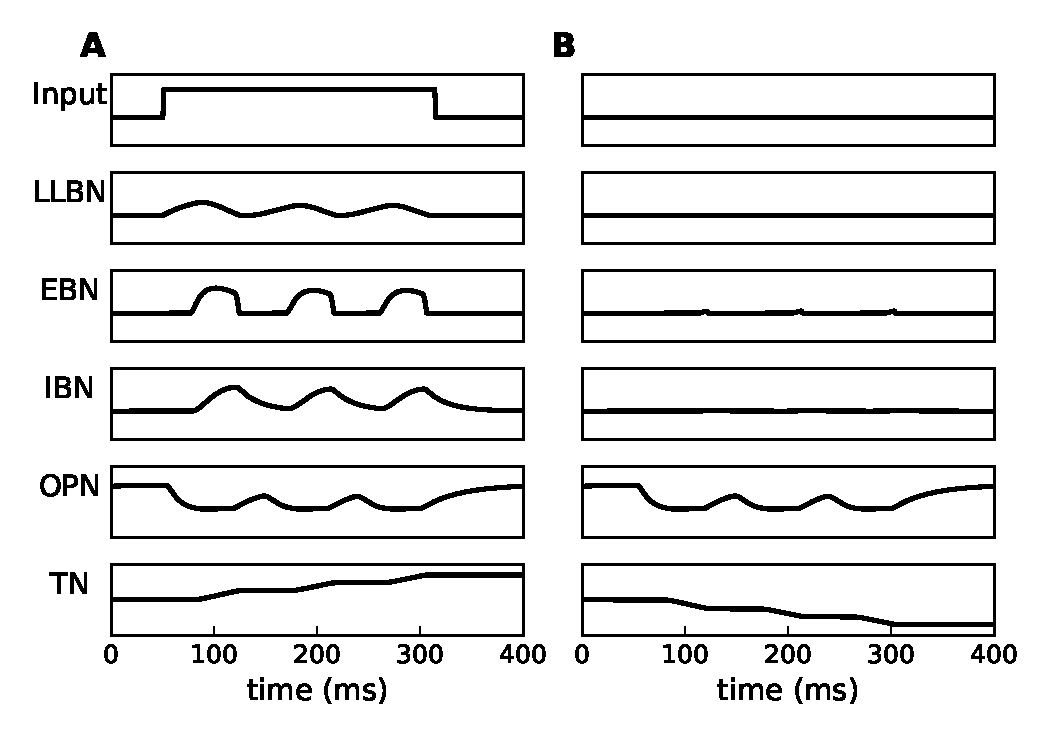
\includegraphics[width=0.75000\textwidth,height=0.45000\textwidth]{figures/fig1.eps}
\caption{\textbf{Activity profiles in the left (A) and right (B) SG.}
All activities are in response to constant input (\(\mathrm{I=1}\))
applied to the left LLBN for \(265\,\mathrm{ms}\).\label{fig:fig_1}}
\end{figure}

The second simulation shows the relation between input strength and
burst amplitude for LLBNs and EBNs. With increasing input strength, both
amplitude and duration of activation increased in long-lead and
excitatory burst neurons. As before, these results accord well with
those shown in figure 5 of the original publication.

\begin{figure}
\centering
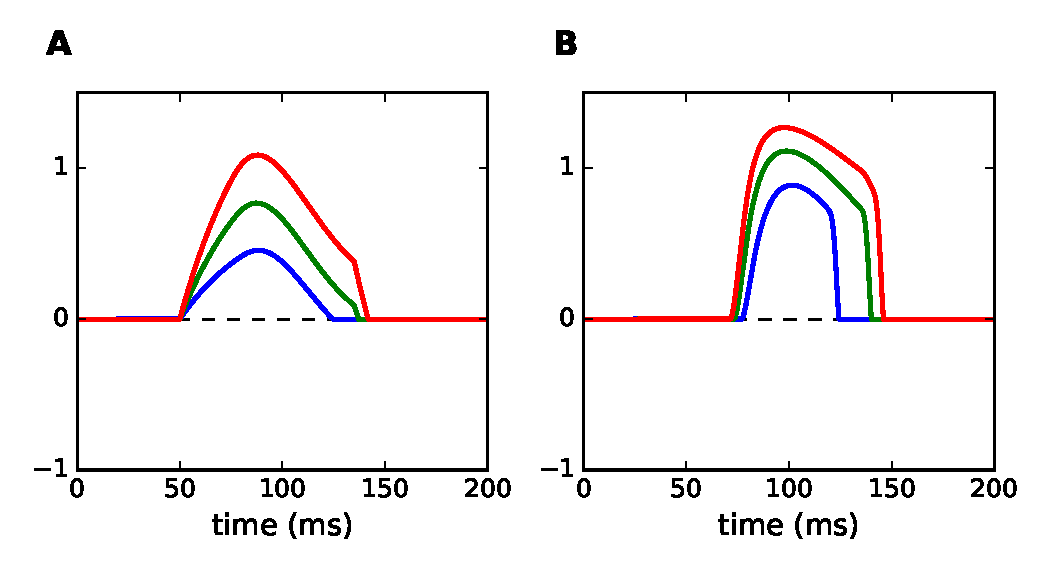
\includegraphics[width=0.75000\textwidth,height=0.36000\textwidth]{figures/fig2.eps}
\caption{\textbf{Activity profiles in LLBN (A) and EBN (B).} Increased
input strength resulted in larger LLBN and EBN burst size with inputs
equal to 1 (blue), 1.75 (green), and 2.5 (red) each applied to the left
LLBN for \(85\,\mathrm{ms}\).\label{fig:fig_2}}
\end{figure}

The third simulation generates saccades in response to different input
strengths applied to the horizontal and vertical SG (figure
\ref{fig:fig_3}). As in the original publication, saccades were
generally straight with a slight tendency to curve. We extracted
quantitative estimates of saccade amplitude for the original publication
from their figure 6 and calculated the root-mean-squared error (RMSE)
between these estimates and saccade amplitudes produced by our model.
The RMSE was 0.16\textdegree, 0.17\textdegree, 0.18\textdegree,
0.22\textdegree, 0.14\textdegree~for the blue, green, red, turqoiuse,
and purple curves, respectively. Given that saccade amplitudes are
between 10\textdegree~and 15\textdegree, these RMSE values indicate a
close match between the two implementations.

\begin{figure}
\centering
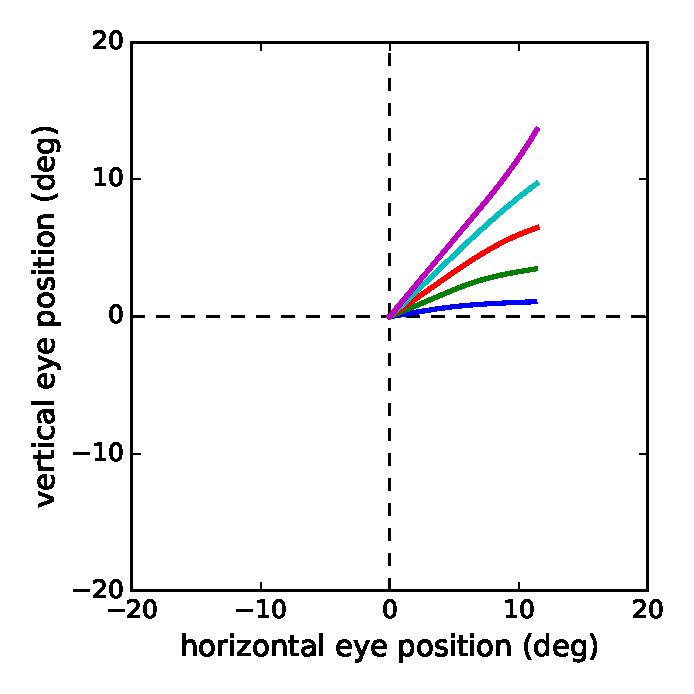
\includegraphics[width=0.48750\textwidth,height=0.48750\textwidth]{figures/fig3.eps}
\caption{\textbf{Oblique saccades.} Inputs to the right and upward LLBNs
were \(\mathrm{{I}_{r}=0.67}\) \& \(\mathrm{{I}_{u}=0.08}\) (blue);
\(\mathrm{{I}_{r}=0.7}\) \& \(\mathrm{{I}_{u}=0.22}\) (green);
\(\mathrm{{I}_{r}=0.74}\) \& \(\mathrm{{I}_{u}=0.4}\) (red);
\(\mathrm{{I}_{r}=0.75}\) \& \(\mathrm{{I}_{u}=0.6}\) (turqoiuse); and
\(\mathrm{{I}_{r}=0.7}\) \& \(\mathrm{{I}_{u}=0.9}\) (purple) and were
applied for \(75\,\mathrm{ms}\). As expected, saccades were fairly
straight with a slight tendency to curve.\label{fig:fig_3}}
\end{figure}

The fourth simulation implements a staircase of three saccades in
response to continuous input (figure \ref{fig:fig_4}). Our results agree
with those reported in the original publication (their figure 7) with
saccades being of equal length and the smaller component (horizontal)
being stretched to produce straight oblique saccades.

\begin{figure}
\centering
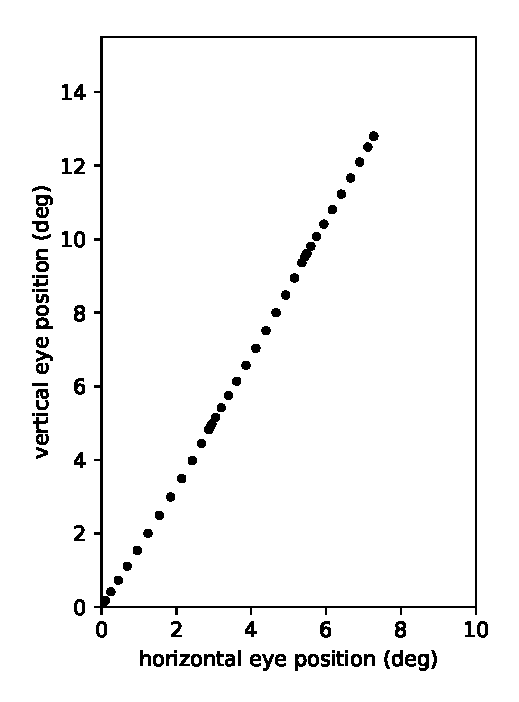
\includegraphics[width=0.33000\textwidth,height=0.45000\textwidth]{figures/fig4.eps}
\caption{\textbf{Saccadic staircase.} Three saccades in a staircase
continued in the same direction as the initial saccade. Inputs to the
right and upward LLBNs were equal to \(\mathrm{{I}_{r}=0.2}\) and
\(\mathrm{{I}_{u}=0.33}\) for \(250\,\mathrm{ms}\). Eye position was
sampled every \(2\,\mathrm{ms}\).\label{fig:fig_4}}
\end{figure}

In the fifth simulation the average activity of the left EBN was
obtained for a series of saccades with different directions. Figure
\ref{fig:fig_5} shows a polar plot of average activity corresponding to
each saccade reflecting the neuron's tuning curve. The tuning curve we
observed for the left EBN exhibits a cardioid-like shape as was the case
in the original publication (figure 8).

\begin{longtable}[]{@{}lllllllllllllll@{}}
\caption{Direction specific inputs to SG to produce EBN tuning curve.
\label{tbl:table_1}}\tabularnewline
\toprule
& 0 & 45 & 72 & 90 & 108 & 135 & 162 & 180 & 198 & 225 & 252 & 270 & 288
& 315\tabularnewline
\midrule
\endfirsthead
\toprule
& 0 & 45 & 72 & 90 & 108 & 135 & 162 & 180 & 198 & 225 & 252 & 270 & 288
& 315\tabularnewline
\midrule
\endhead
\(\mathrm{{I}_{l}}\) & .00 & .00 & .00 & .00 & .20 & .45 & .63 & .70 &
.63 & .45 & .20 & .00 & .00 & .00\tabularnewline
\(\mathrm{{I}_{r}}\) & .70 & .45 & .20 & .00 & .00 & .00 & .00 & .00 &
.00 & .00 & .00 & .00 & .20 & .45\tabularnewline
\(\mathrm{{I}_{d}}\) & .00 & .00 & .00 & .00 & .00 & .00 & .00 & .00 &
.20 & .45 & .63 & .70 & .63 & .45\tabularnewline
\(\mathrm{{I}_{u}}\) & .00 & .45 & .63 & .70 & .63 & .45 & .20 & .00 &
.00 & .00 & .00 & .00 & .00 & .00\tabularnewline
\bottomrule
\end{longtable}

\begin{figure}
\centering
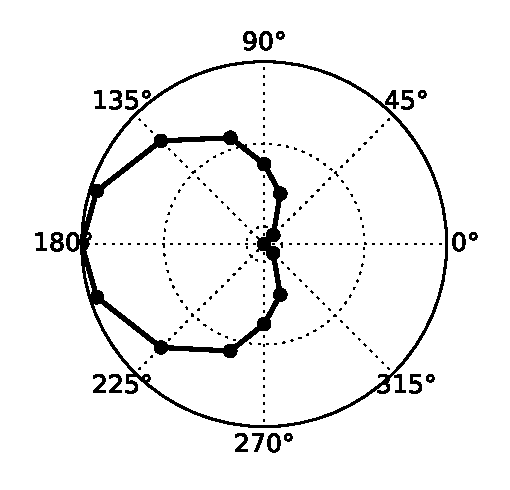
\includegraphics[width=0.37500\textwidth,height=0.37500\textwidth]{figures/fig5.eps}
\caption{\textbf{EBN tuning curve.} Tuning curve of the left EBN
exhibiting a cardioid-like shape. Inputs to the SG producing the desired
saccades can be found in table \ref{tbl:table_1}. Each of these inputs
was applied for \(50\,\mathrm{ms}\).\label{fig:fig_5}}
\end{figure}

\pagebreak
The sixth simulation reported in the original publication was designed
to replicate results of Stanford \textit{et al.}
\autocite{Stanford1996}. These authors stimulated the superior
colliculus (SC) at various frequencies and measured the resulting
saccade amplitude, duration, and velocity; showing that ampltidude
saturates before velocity. Our implementation of the SG model was
capable of replicating these results. However, reproducing simulation
results reported by Gancarz \& Grossberg \autocite{Gancarz1998} with our
implementation was complicated by the fact that the stimulation protocol
given by the authors lead to the production of two rather than a single
saccade for larger stimulation intensities. Furthermore, the authors did
not report their criteria for identifying saccade on- and offsets.
Stanford \textit{et al.} \autocite{Stanford1996} used velocity criteria
to determine onset (\(v\textgreater30\,\mathrm{deg/s}\)) and offset
(\(v\textless30\,\mathrm{deg/s}\)) of a saccade. While this provided us
with explicit criteria, velocity did not always drop below
\(30\,\mathrm{deg/s}\) after the first saccade before rising again with
the second. To determine the offset of a saccade in those cases, we
found the local minimum between the end of the first and the beginning
of the second saccade. With these criteria in place, we stimulated the
SC. Results of our simulation are shown in figure \ref{fig:fig_6}. We
extracted quantitative results of the original publication from their
figure 9 and calculated the RMSE between these estimates and our results
for each curve. The RMSE was 1.24\textdegree, \(0.46\,\mathrm{ms}\), and
\(4.45\,\mathrm{deg/s}\) for saccade amplitude, duration, and peak
velocity, respectively. Our results accord thus very well with those
reported in the original publication. This includes the observation that
saccade amplitude and especially saccade duration were largest for a
stimulation intensity of 1.2. It is conceivable that this intensity
marks the point after which the SG generator starts producing two rather
than a single saccade with the eye movement at this intensity merging
two saccades and thus being stretched out.

\begin{figure}
\centering
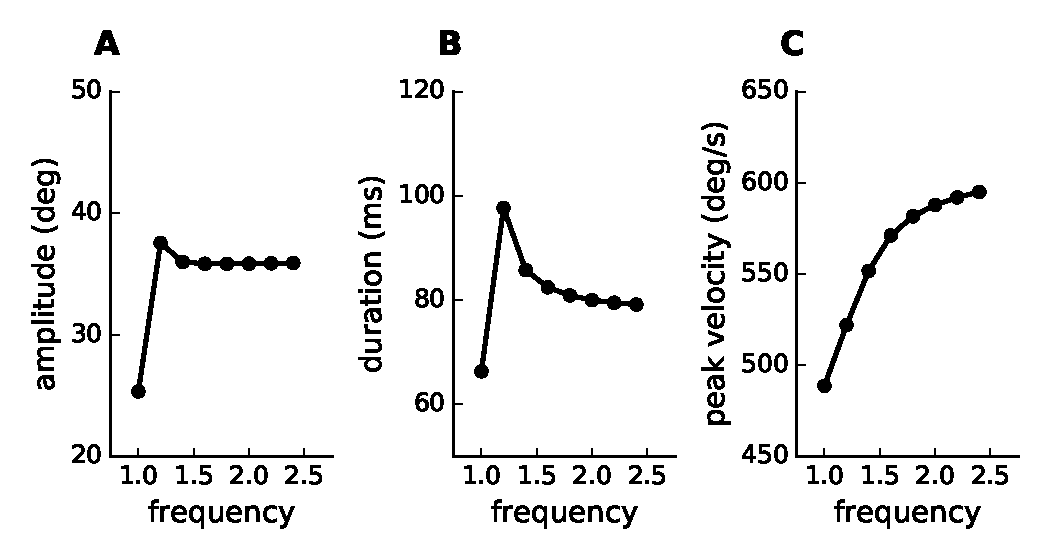
\includegraphics[width=0.75000\textwidth,height=0.37500\textwidth]{figures/fig6.eps}
\caption{\textbf{Effect of stimulation frequency on saccade (A)
amplitude, (B) duration, and (C) velocity.} Saccade amplitude (A)
saturated before saccade velocity (C). A range of unitless values
varying between 1 and 2.4 at increments of 0.2 were applied to the SC
(reflecting stimulation at different frequencies). The connection weight
from SC to LLBN was \(\mathrm{W=2}\) and stimulation duration was
\(125\,\mathrm{ms}\).\label{fig:fig_6}}
\end{figure}

\begin{figure}
\centering
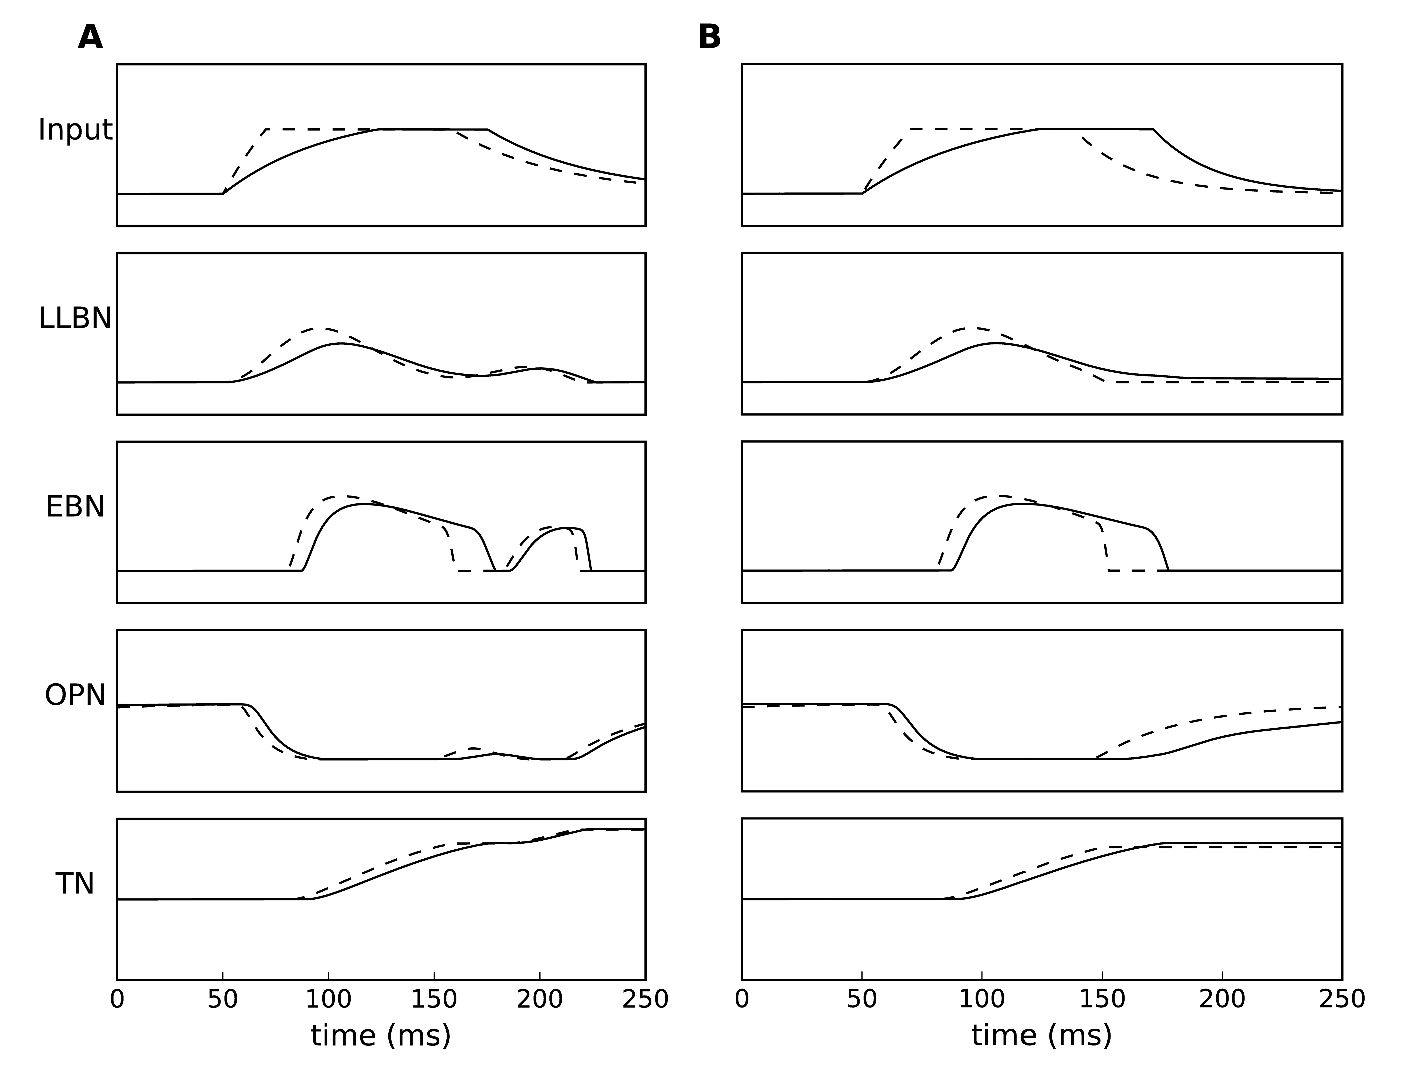
\includegraphics[width=0.90000\textwidth,height=0.90000\textwidth]{figures/fig7.eps}
\caption{\textbf{Trading saccade velocity for duration.} Duration and
velocity of a saccade can be traded while keeping amplitude constant. To
produce a high velicity saccade an input of \(\mathrm{F=3}\) was applied
to the SC for \(68\,\mathrm{ms}\) (\(82\,\mathrm{ms}\) in the original
publication). To produce a low velicity saccade an input of
\(\mathrm{F=1.3}\) for \(117\,\mathrm{ms}\). Given the shape of the
input curve produced by our implementation of the original equations
(A), a second saccade can be observed for both high and low velocity
saccades. If the input curves reported in the original manuscript were
recreated in an ad-hoc fashion (B), the responses of all model neurons
matched those in \autocite{Gancarz1998}\label{fig:fig_7}}
\end{figure}

\begin{figure}
\centering
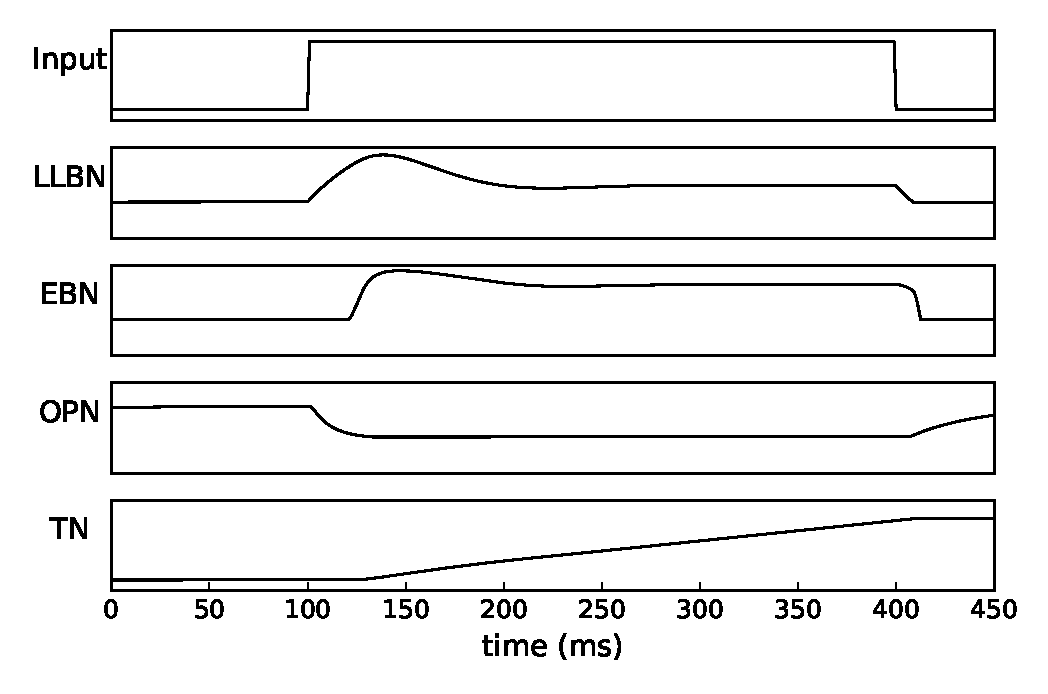
\includegraphics[width=0.70000\textwidth,height=0.56200\textwidth]{figures/fig8.eps}
\caption{\textbf{Smooth staircase eye movements.} Activity profiles of
SG neurons accompanying smooth eyes movement as a result of strong
(\(\mathrm{I=3}\)) sustained (\(300\,\mathrm{ms}\))
input.\label{fig:fig_8}}
\end{figure}

\begin{figure}
\centering
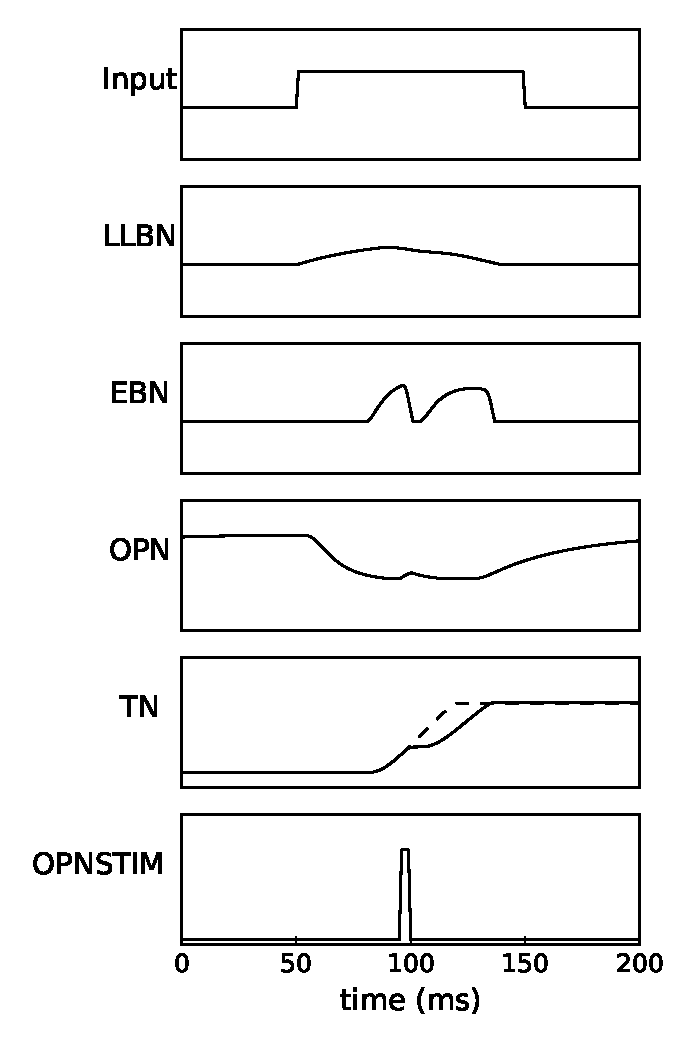
\includegraphics[width=0.46200\textwidth,height=0.60000\textwidth]{figures/fig9.eps}
\caption{\textbf{Interrupted saccade resulting from OPN stimulation.}
OPN stimulation interrupted the saccade, which remained accurate
nonetheless. An input of (\(\mathrm{I=0.7}\)) was applied to the LLBN
for \(100\,\mathrm{ms}\). At \(45\,\mathrm{ms}\) after onset of the
input, the OPN was stimulated (\(\mathrm{J=1.8}\)) for
\(5\,\mathrm{ms}\). The dashed line shows TN activity for an
uninterrupted saccade.\label{fig:fig_9}}
\end{figure}

The seventh simulation shows that saccade velocity and duration can be
traded while keeping amplitude constant. To produce a high-velocity
saccade, the SC was stimulated at a high frequency. Similarly, to
produce a low-velocity saccade, the SC was stimulated at a low
frequency. Figure \ref{fig:fig_7} shows the results of our simulation.
In line with the original publication, the saccade amplitude reflected
by TN activity was identical after high- and low-frequency saccades thus
confirming the reported effect. However, we observe differences in the
specific details of our implementation with respect to the original,
starting with the shape of the input curves. While the rise of the input
curves in the original publication and our implementation coincide well,
the decay in our curves started later and proceeded with a shorter time
constant (\(\approx25\,\mathrm{ms}\), i.e.~half the simulation time
constant). This resulted in more total input to the model in our
implementation and hence lead to the generation of a second saccade not
observed in the original publication. When repeating our simulation
using an ad-hoc solution to create matching input curves (by halving the
time constant after external stimulation), we observed results identical
to those reported in the original publication. We proceeded to
investigate the origin of the discrepancy with regard to the shapes of
the input curves. First, we tested whether discrepancies were specific
to our NEST implementation by solving the expressions describing the
input analytically. Specifically, the analytic expression of the input
\(I(t)\) described by equations \ref{eq:sc} - \ref{eq:stim} is
\begin{equation}
I(t)=
\left\{
\begin{array}{lll}
    0 \quad &\textrm{if} \quad t<{t}_{on} \\
    W \cdot f(F \cdot (1-{e}^{-(t-{t}_{on})/ \tau})) \quad &\textrm{if} \quad {t}_{on}<t<{t}_{off} \textrm{.}\\
    W \cdot f(F \cdot (1-{e}^{-({t}_{off}-{t}_{on})/ \tau}) \cdot {e}^{-(t-{t}_{off})/ \tau}) \quad &\textrm{if} \quad t \geq {t}_{off} \\
\end{array}
\right.
\label{eq:analytic}\end{equation} Evaluating the analytic expression
given parameter values reported in the original manuscript exactly
reproduced our numerical results and thus produced curves equally
deviating from those shown in the original publication. Next, we
contacted one of the original authors to rule out the possibility that
we used erroneous parameter settings but no mistake was pointed out to
us. The origin of the discrepancy thus remains unclear. However, it is
likely it stems from the description of the input rather than from
problems with the SG model itself.

The eighth simulation reported by Gancarz \& Grossberg
\autocite{Gancarz1998} shows how strong sustained input to the SG
produces smooth eye movements. Our results, shown in figure
\ref{fig:fig_8}, reproduced these findings as they strongly resembled
those shown in figure 11 of the original publication. Specifically, an
initial burst exhibited by the EBN was followed by sustained lower
activity. This was due to inhibitory feedback being insufficient to
silence the LLBN when input remains continuously strong and resulted, in
turn, in the observed smooth eye movement.

The final simulation showcases the evolution of activity exhibited by SG
neurons when the OPN is briefly electrically stimulated while a constant
input is applied to the LLBN. External stimulation temporarily restored
activation in the OPN and hence also inhibition of the EBN, leading to
an interruption of the saccade. As is shown in figure \ref{fig:fig_9},
the saccade remained accurate despite this disruption. This is in
agreement with results shown in figure 12 of the original publication.

\section{Conclusion}\label{conclusion}

The reproduced results show very good qualitative correspondence with
those reported by Gancarz and Grossberg \autocite{Gancarz1998} and
accorded well quantitatively whenever such information was available.
The only discrepancy between our and the original implementation was
that the input to the saccade generator took more time to decay in our
implementation. While the exact cause of this discrepancy is unclear, we
could rule out that it was specific to the NEST implementation.
Furthermore, it does not affect reproduction of the main finding of
simulation seven; namely that saccade velocity and duration can be
traded while keeping its amplitude constant.

In conclusion, our reproduction confirms the results of the original
publication and shows that an implementation in the NEST framework is
feasible. This allows for the straightforward integration of the saccade
generator with computational models of other components of the
visuo-motor system (e.g.~salience computation) within a shared
framework.

\section{Acknowledgments}\label{acknowledgments}

All network simulations carried out with NEST
(http://www.nest-simulator.org). This research was funded by the
European Union's Horizon 2020 Research and Innovation Programme under
Grant Agreement No. 7202070 (HBP SGA1).

\section{Appendix}\label{appendix}

\subsection{A1 - Rate neurons in NEST}\label{a1---rate-neurons-in-nest}

For a detailed, comprehensive, treatment of rate-based neuron models in
NEST see Hahne et al.\autocite{Hahne2017}. Here we provide only a brief
overview to facilitate readability/interpretability of the code provided
with this publication. In general, rate-based neurons in NEST consist of
two components; a neuron and a gain function.

\subsubsection{Neuron}\label{neuron}

Two types of neuron base classes exist in NEST v2.16.0:
\texttt{rate\_neuron} and\\
\texttt{rate\_transformer\_node}. The \texttt{rate\_neuron} implements
continuous rate dynamics with and without multiplicative coupling. It
can apply a nonlinear gain function to its inputs either before or after
their weighted summation. It is numerically integrated using the EE
method unless a neuron does not exhibit exponential decay in which case
the EM method is used. Furthermore, rates can be bounded (from below at
zero) or unbounded. Finally, noise (in the form of a Wiener process) can
be added to its input or to its output. The \texttt{rate\_neuron} has a
total of seven parameters (see table \ref{tbl:table_2}) and two further
properties \texttt{rate} (current firing rate) and \texttt{noise}
(current noise level).

\begin{longtable}[]{@{}lll@{}}
\caption{\texttt{rate\_neuron} parameters.
\label{tbl:table_2}}\tabularnewline
\toprule
parameter & default value & description\tabularnewline
\midrule
\endfirsthead
\toprule
parameter & default value & description\tabularnewline
\midrule
\endhead
\texttt{tau} & \(10\,\mathrm{ms}\) & time constant\tabularnewline
\texttt{lambda} & \(1\) & passive decay rate\tabularnewline
\texttt{std} & \(1\) & noise standard deviation\tabularnewline
\texttt{mean} & \(0\) & mean firing rate\tabularnewline
\texttt{linear\_summation} & \texttt{true} & if true, apply gain
function after summation\tabularnewline
\texttt{rectify\_output} & \texttt{false} & if true, multiplicative
coupling\tabularnewline
\texttt{mult\_coupling} & \texttt{false} & if true, rate is
bounded\tabularnewline
\bottomrule
\end{longtable}

For the implementation of this neuron see
\texttt{rate\_neuron\_ipn\_impl.h} and\\
\texttt{rate\_neuron\_opn\_impl.h} in
\texttt{../nest/nest-simulator-master/models} for input and output
noise, respectively.

The \texttt{rate\_transformer\_node} instantaneously applies a
nonlinearity to its inputs but does not exhibit temporal dynamics. It
can be used to apply different nonlinearities to different inputs to a
single neuron. This class has only the \texttt{rate} property and no
parameters. For its implementation see
\texttt{rate\_transformer\_node\_impl.h} in
\texttt{../nest/nest-simulator-master/models}.

\subsubsection{Gain function}\label{gain-function}

Five gain functions exist in NEST v2.16.0: \texttt{lin\_rate},
\texttt{sigmoid\_rate},\\
\texttt{sigmoid\_rate\_gg\_1998}, \texttt{tanh\_rate}, and
\texttt{threshold\_lin\_rate}. Documentation of each gain function is
given in the header file with the corresponding name within
\texttt{../nest/nest-simulator-master/models}. We added
\texttt{sigmoid\_rate\_gg\_1998} specifically for the reimplementation
of the saccade generator presented here.

Gain functions are combined with a neuron class to obtain a specific
neuron model. For instance, the combination of the \texttt{lin\_rate}
gain function with the \texttt{rate\_neuron\_ipn} class gives the
\texttt{lin\_rate\_ipn} neuron model. The parameters of a model are a
combination of all parameters of the neuron base class and all
parameters of the gain function. Within Python the command
\texttt{nest.Models()} lists all existing model types including all
implemented combinations of gain function and neuron class.

{\sffamily \small
  \printbibliography[title=References]
}
\end{document}
